\documentclass[11pt, a4paper]{article}
\usepackage{graphicx}
\graphicspath{ {images/} }
\usepackage{geometry}
\usepackage{multicol}
\usepackage{float}
\usepackage{mathtools}
\usepackage{python}
  \geometry{
 a4paper,
 total={170mm,257mm},
 left=20mm,
 top=20mm,
 }
\title{Development of a database for statistical analysis and classification of X-ray diffraction datasets}
\author{Dominic Jaques\\ Diamond Light Source, Ltd.\\ Supervised by Dr. Melanie Vollmar and Mr. James Parkhurst}
\begin{document}
\maketitle
\section{Introduction}
The purpose of the project was to construct a database with a Python API, in order to interact with the metadata, for the collection of standard datasets from x-ray diffraction images to be used for statistical analysis, looking at trends within datasets and classification of datasets using certain statistical indicators. The derived statistics are then to be used in machine learning code to train models to predict processing success of crystallographic diffraction data. 
\vspace{5mm}
\begin{multicols}{2}
\section{Theory} 
\subsection{Databases}
A database, by it's simplest definition, is ``a collection of pieces of information that is organised and used on a computer''$^{[1]}$ and is usually designed to cater for a large collection of data organised to allow for fast read and write time for a computer. Most databases are built upon a database management system (DBMS) which is a platform that already allows for a user to construct and interact with a database using special purpose languages, typically the ``Structured Query Language'', SQL. DBMSs support different database models but the most commonly used model, and the one used for this project was the relational model.
\subsubsection{Relational Model}
This approach of managing data represents all data in terms of tuples (rows) and attributes (columns), grouped into relations (tables)$^{[2]}$. It allows for a declarative method of querying and selecting data; the user provides the information that the database contains and states directly what they want to retrieve from it. Most databases function using the SQL data structure, and use its query language. Tables are made that categorise data in order to minimise repeated fields. Each table relates to a specific entity and then points to a parent table that contains more information relating to another entity, that may or may not encompass the original. The important point is that the data is not repeated in any table. A good example of this is music: the track table contains information on the song, e.g. length and track title, and each track in the table also points to a row in a different table, the album table, which contains more information pertaining only to the album, e.g. album title and number of songs. By removing replicated data and replacing it with references to a single copy of each bit of data we build a ``web'' of information that the relational database can read through very quickly  - even for large amounts of data$^{[3]}$. This reference system, or web, is set up using a system of keys: the primary key, foreign key, and logical key. 
\begin{figure}[H]
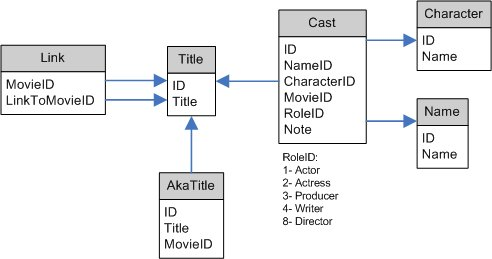
\includegraphics[width = 7cm]{datastructure_converted}
\caption{\footnotesize An example of a relational database demonstrating the concept of primary and foreign keys. The foreign key in one table, say \textit{MovieID} in the \textit{Link} table, points to the primary key in another table, the \textit{ID} column in the \textit{Title} table.$^{[4]}$}
\centering
\end{figure}
The primary key is a unique identifier, normally an integer, that is auto generated by the DBMS as an attribute in a table. It must be unique since each key refers to one and only one row. The purpose of the foreign key, which is entered manually, is to then `point' where two rows in separate tables are related. If, as in the example above, one row in the \textit{Link} table is related to a row in the \textit{Title} table then we assign the foreign key according to:
\begin{equation*}
\text{Foreign Key} = \text{Primary Key}.
\end{equation*}
The logical key is simply the main key that a human might be interested in, e.g. ``Movie Title'', but to the DBMS it is just another field. 
\subsubsection{SQL}
As mentioned before, SQL is a special purpose language designed for interacting with database software. The scope of SQL includes data insert, query, update, delete, schema creation and modification, and data access control.
\begin{figure}[H]
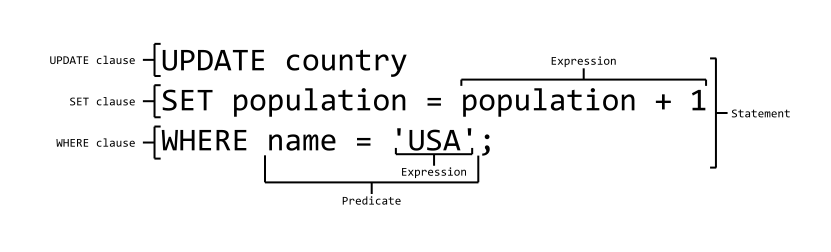
\includegraphics[width = 5.5cm]{sql}
\centering
\caption{\footnotesize A labeled figure of the many language elements that make up an SQL Statement.$^{[5]}$}
\end{figure}
Using libraries native to Python these SQL statements can be executed from within a Python script.
\subsection{Machine Learning}
The subject of Machine Learning is incredibly broad and detailed and so could not possibly be covered here in enough summary to fully explain or give motivation to all the methods that will follow. This will merely be a mathematical outline of how the classifier will be built. 
\\
\\Since each set of data acquired through x-ray diffraction relates to one attempt at phasing we can reduce our problem down to the following: for a dataset $X$ we want to make a prediction $y \in \{0,1\}$ as to whether or not we will be able to perform phasing successfully. We need a mathematical model that converts the statistical indicators in $X$ into a number between 1 and 0, relating to how likely they are to be successful. We do not know the form of this model, and so want to train an algorithm to pick the best one. The normal method associated with this requires two matrices, the ``feature matrix'' $X$ and the ``parameter matrix'' $\theta$.
\begin{equation*}
X = \begin{bmatrix} x_1 \\ x_2 \\ \vdots \\ x_n \end{bmatrix}, \quad 
\theta = \begin{bmatrix} \theta_1 \\ \theta_2 \\ \vdots \\ \theta_n \end{bmatrix}
\end{equation*}
The elements of the matrix $X$ are all of the possible features that could help predict the outcome. These could be simply all the numerical values of the related statistics, however they could be more complex such as polynomials or combinations of two different features. The matrix $\theta$ is much simply and just accounts for the weighting of each related feature (each element is the coefficient of the predicting features). We define our model as
\begin{equation*}
\theta^T X = \theta_1 x_1 + \theta_2 x_2 + \cdots + \theta_n x_n.
\end{equation*}
It should be noted that in reality we will pick many different models, e.g.:
\begin{itemize}
\item$\theta_1 x_1 + \theta_2 x_1^2 + \theta_3 x_2 + \cdots + \theta_n x_n$
\item$\theta_1 x_1 + \theta_2 x_1x_2 + \cdots + \theta_n x_n$
\item$\vdots$
\item$\theta_1 x_1^2x_2 + \theta_2 x_1x_2x_3 + \cdots + \theta_n x_n$
\end{itemize}and put them all through the following process.\\
We pass all our models through the following hypothesis:
\begin{equation*}
h_\theta(X) = \frac{1}{1+e^{-\theta^TX}}
\end{equation*}
known as the ``logistic'' function that has the following form.
\begin{figure}[H]
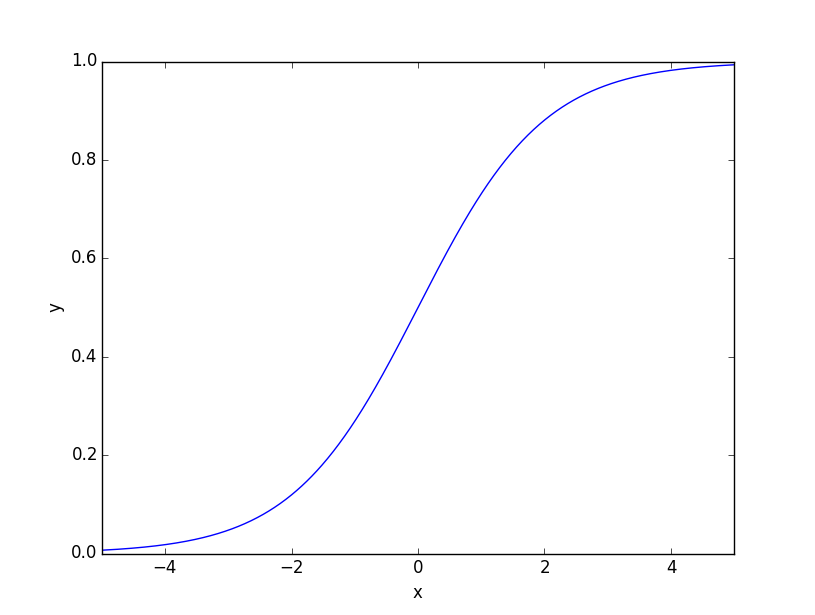
\includegraphics[width = 5cm]{sigmoid}
\centering
\caption{\footnotesize Form of the sigmoid function, bound between 0 and 1, giving an estimation of probability.}
\end{figure}
The parameter vector should now be optimised using a training set of data (data with known solutions) that gives us the best fit. We measure this using the cost function, $J(\theta)$:
\begin{equation*}
 J(\theta) = \frac{1}{2m}\sum^m_{i=1}(h_\theta(x^{(i)})-y^{(i)})^2
 \end{equation*}
 where the superscript $(i)$ counts which set of data we are using. This function sums up the difference between the value outputted by our model and the actual result (a 0 or 1), meaning the larger it is the worse the model is. The feature vector is then updated according to
\begin{equation*}
\begin{aligned}
\text{Repeat for } j=1 \to n \quad \{ & \\
 \theta_j &:= \theta_j - \alpha \frac{\partial}{\partial \theta_j} J(\theta) \\
& \}
\end{aligned}
\end{equation*}
which brings the model to the nearest minimum in the cost function. This can be repeated for all models of $\theta^TX$ until we find one with the lowest $J(\theta)$ and can conclude this as the best fit algorithm.$^{[6]}$
\section{Method}
The goal of the project was to construct a database for the collection of standard datasets that would be lightweight enough for easy setup and use, by any user. The database would be used for looking at trends within datasets and classification of datasets using certain statistical indicators. The derived statistics are to be used in machine learning code to train models to predict processing success of crystallographic diffraction data. The work was done in the following stages: Given a set of existing X-ray diffraction datasets, a database was be created that retrieved information from data directories and tables for the various metadata and statistics. This was accomplished through the development of a Python language API  and a set of corresponding command line utilities were later introduced for interacting with the database. In particular the API includes functions for adding a single new dataset and its corresponding metadata to the database or an entire directory's worth. The design of the API was kept as flexible as possible to allow additional scripts and processing statistics to be added in future. The database will be used to query the different datasets to try and determine trends and correlations between dataset statistics. Work has begun on using the derived data for processing statistics to train prediction functions which are based on neural networks and machine learning algorithms, the rough method of which is outlined in section 2.2 Machine Learning.
\subsection{Building the database}
The desired structure of the project was to have a series of command line utilities that executed scripts written in Python and embedded in those scripts would be SQL statements that would interact with the database directly, stored locally as an sqlite file.
\begin{center}
\begin{tabular}{|c|}
\hline\\
\quad Command Line \quad \\
\\
\hline \\
\quad Python API  \quad \\
\\
\hline \\
SQL \\
\\
\hline 
\end{tabular}
\end{center}
The procedure that was followed in general was:
\begin{enumerate}
\item  Identify a new feature required for the database.
\item Build a python script to acquire any necessary data for this feature.
\item  Implement SQL statements into the script that would alter/update the database as required.
\item  Execute and interact with the database.
\end{enumerate}
\subsubsection{Database Initialisation}
In order to update and populate the database it first needed to be set up, which requires a script that constructs the schema of the database. The schema was planned to be lightweight and to allow for easy data extraction by limiting the path length of related data that would likely be extracted at the same time. Any script wishing to interact with the database must do so by the following:
\begin{verbatim}
import sqlite3
conn = sqlite3.connect(`metrix_db.sqlite')
cur = conn.cursor()
\end{verbatim}
This handle can now be used in order to execute SQL commands to add tables to the database. A schema was devised that would contain the basic statistics of a sweep, extracted from the xia2\footnote{an image and data processing software application for x-ray diffraction images.} processing pipeline and also reference statistics from a pdb file. The end result:
\begin{figure}[H]
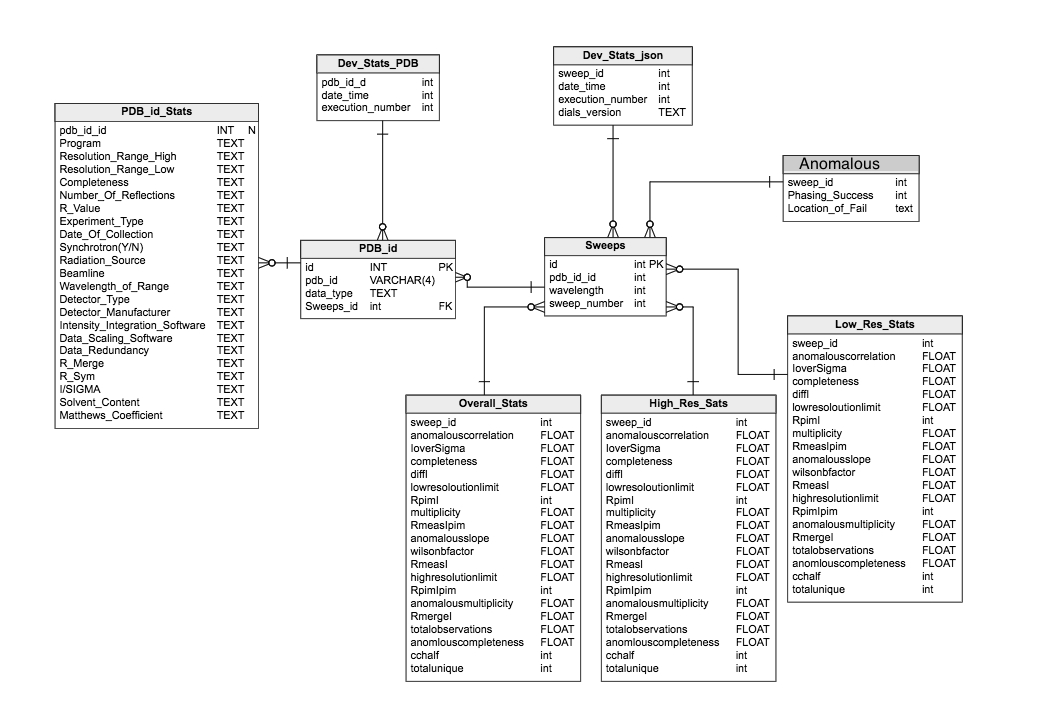
\includegraphics[width=8cm]{metrix_database}
\centering
\caption{\footnotesize The database schema that was devised for the project. There were several discussions on what data was considered necessary which is what lead to the two developer tables, that give reference information on when data was inputted into the database.}
\end{figure}
 The next step was then to create each table in schema and link any keys to one another. The `central' table was decided to be the PDB id table, which would contain just the PDB id and act as a label on which to join the necessary data. This is all included in the script titled `table\_initialise.py'
\begin{verbatim}
cur.execute(```
CREATE TABLE PDB_id (
    id INTEGER PRIMARY KEY AUTOINCREMENT 
       UNIQUE,
    pdb_id TEXT UNIQUE
)''')
\end{verbatim}
We declare in SQL we wish to make a table called `PDB\_id' that has columns 'id' and 'pdb\_id'. The arguments following each of the column headings are instructions to the DBMS on how it should treat these columns. They are self explanatory, but it should be noted by labelling a column as unique you tell the DBMS to throw an error if the same PDB id is attempted to be reinserted into the database. The other tables were initialised using the same format. 
\subsubsection{Populating the database}
After having set up the skeleton of the database data needed to be added to it. The reference statistics found in the PDB data files were considered to be the ideal starting place as they were all available and easily readable. A script was setup, `pdb\_parsery.py', that searched a directory containing pdb files and would then open and read these files, scanning each line for indicators of required statistics and would then extract the value associated with this statistic.
\begin{verbatim}
def lineCheck(wordlist, line):
    wordlist = wordlist.split()
    return set(wordlist).issubset(line)

def statRetreive(line):
    try:
        pos = [i for i,x in enumerate(line) 
                                if x == ':']
        return ' '.join(line[-1:])
    except:
        print 'Could not find data for: 
                                %s' % (line)
\end{verbatim}
These were the two functions used in order to find the right line and then to extract the correct value from it. This data was was then stored in a dictionary where the associated key was the column heading of that value. By storing the values all in a dictionary it allowed to insert the data into the database using a recursive loop, greatly reducing the amount of repeated code.
\begin{verbatim}
for data in pdb_data:
    cur.execute('''
    UPDATE PDB_id_Stats 
    SET "%s" = "%s"
    WHERE pdb_id_id = "%s" ''' % 
               (data, pdb_data[data], pdb_pk ))
\end{verbatim}
The second set of data to start inserting, and the main purpose of the project, were the x-ray diffraction datasets that came through processing from xia2. This required opening and extracting data from json files. The data required from the file was several levels down in the hierarchy and so required a lot of file handle manipulation. In the script, `json\_parser.py', it often gets quite difficult to read where in the file the data is coming from. For purposes of readability the data was always taken from the file and placed into lists within Python, rather than using the handle to the file directly. Once this data was extracted it could then, as before with the pdb statistics, be recursively added into the database.\\
\\
At this point in the project the database could be initialised and populated with both reference statistics and diffraction datasets using three different scripts in the developing Python API.
\subsubsection{Feature Tables}
Additional features were added to the database, which can be seen in Figure 4, these were development tables and an anomaly table. The development tables contain auto generated values that are either produced as the database is update or are extracted from the metadata of the related files. Presently they contain the time of insertion of the data, the execution number (how many times the same dataset has been inserted into the database), whether the data was parsed successfully (if there were missing files or a broken file structure), and the version of processing software used to get the diffraction datasets. As an experiment of concept these feature tables were added in two ways.
\begin{enumerate}
\item Editing the initialisation script in order to directly build the tables from the outset.
\item Building a new script (`anomaly\_table.py') that creates a new table on the database and adds data to it.
\end{enumerate}
Item 2 was trialled in order to see how easy the database will be to alter in the future with some repurposing script. Item 1 is the preferred method for further alterations to the mainframe of the database in the future and item 2 should be used for additions of features that will not be general purpose, since not all users will be using the database for the same reason and may not always activate all scripts, thereby possibly missing fully completing the database. This evaluation will be included again later. 
\subsubsection{Viewing and exporting the data}
In order to view the database there are two available options. The first, and strongly advised, is to download a database visualisation software such as ``sqlitebrowser''$^{[7]}$, the one used for this project. This allows the user to easily see the data structure, manually interact with the data, and to export the data. The alternative option is to export the required data using the `csv\_constructor.py'. This script exports the fields and tables prompted by the user to a csv file. This is not the advised way to view data in the database as it is not guaranteed to produce the data in an easily readable format. A browsing software application is \textit{strongly} recommended. The csv constructor script is designed so that a user may export data from the database in order to be able to perform statistical analysis on it, and for use use as training sets for machine learning algorithms. 
\subsection{Machine Learning}
Due to time limitations towards the end of this project development of this section was limited, although extensive preparation and research was done. The contribution of this project towards the training of the machine learning algorithm is found within the script `phasing\_success.py'. This scans the log files of the xia2 processing output in oder to check whether or not it was successful in phasing. The script then updates the database accordingly in the table 'Phasing' as either a 1 or 0 depending on the success of the dataset. This, coupled with the csv constructor allows a user to export the database as a csv file with columns of the required statistics and of the success. Resultantly using the Python libraries `pandas' and `numpy' we can convert the columns of statistics into the array $X$ and the column of 1s and 0s into the array $y$, allowing the user to begin supervised learning algorithms. 
\section{Functionality}
The current API consists of the following scripts, organised in the order of advised execution.
\begin{itemize}
\item table\_initiliase.py
\item pdb\_id\_writer.py
\item pdb\_parser.py
\begin{itemize}
\item single\_pdb\_parser.py
\end{itemize}
\item json\_parser.py
\begin{itemize}
\item single\_json\_parser.py
\end{itemize}
\item anomaly\_table.py
\item phasing\_sucess.py
\item csv\_constructor.py
\end{itemize}
To view the database some database management software is required. The advised application is 'sqlitebrowser'. All of the data processing scripts can take a directory command line argument using `--directory=your/file/path', the current default directories are the ones that were used in the development of the project. The database is designed to be set up in a few simple steps.
\begin{enumerate}
\item table\_initiliase.py\\
- This builds the 'metrix\_db.sqlite' file and constructs the database schema.
\item pdb\_id\_writer.py\\
- This scans the directory for any files with a directory title that is a PDB id and adds them to a txt file that will be opened and used by the json\_parser.py script. 
\item pdb\_parser.py\\
- This adds all the reference statistics from pdb files in the directory specified in command line or the default directory is currently '/dls/mx-scratch/jcsg-data/PDB\_coordinates'. This step is not necessary if reference statistics are not needed.\\
- The script single\_pdb\_parser.py can be used instead, adding only one entry when provided with a PDB id and directory in the command line using '--pdb\_id=' and '--directory='. 

\item json\_parser.py\\
- This extracts statistics from the xia2 processing files in the directory specified in command line using '--directory='. The default directory is currently /dls/mx-scratch/melanie/for\_METRIX/data\_base\_ proc'.\\
- The script single\_json\_parser.py can be used instead, adding only one entry when provided with a PDB id and directory in the command line using '--pdb\_id=' and '--directory='. 
- Note: This script calls on the file 'pdb\_id\_list.txt' which is a list of the relevant PDB ids in the file.

\item phasing\_success.py\\
- This examines data files in the provided directory and updates the database by labelling each found PDB with a 0 or a 1 depending on whether it has been successful in phasing.\\
\\
The database is now set up and should have all the information that a user would desire.

\item csv\_constructor.py
- This will extract the required information into a csv file format either for viewing or data processing.
\end{enumerate}
\section{Discussion}
The database is functional and can be used to produce processable data and work towards the machine learning algorithm has begun. The discussion will be on noteworthy points in the scripts of the API with the aim to assist further development.
\subsection{Table Initialisation}
Any further work on the mainframe of this database should be done on this script. To add a new table there are two SQL commands that need to be implemented. They are:
\begin{verbatim}
DROP TABLE IF EXISTS Table_Name
\end{verbatim}
and
\begin{verbatim}
CREATE TABLE Table_Name (
variable1 VARIABLE TYPE,
variable2 ...,
...
)
\end{verbatim}
With the relevant key and relational fields entered manually. This first checks to make sure no duplications are being made while the second is the command that constructs the table, with all of the specified information. It should be self evident how to construct these commands from the ones that are already present in the script. 
\subsection{Statistics from PDB files}
The script searches through each specified PDB file and extracts the statistics by searching for indicative words and then returning the last item in the line. There are several functions defined for this and if more statistics are needed in the future they can be found using the same format as those already in the script. There were some issues with statistics coming up in multiple fields/categories so one was selected and the others ignored using an if statement that checked for certain words in the lines. 
\subsection{Processed statistics}
The processed statistics are extracted from a json file in the output files of the xia2 processing. They are found several dictionaries down under ``\_scalr\_statistics.'' The full address of the data varies depending on how the data was collected (SAD, MAD or MR) and the scripts are set up to search for each type. Since this data structure is unique to each type of collection it is also the means by which the data is classified. At the beginning of each successful data pull the variable ``data\_type'' is assigned the title of the data type. Overall this script proved largely time consuming to produce as searching for the specific location and exact data setup proved to be difficult to analyse, but the script does now pull the data from all types of processing and correctly inserts them into the database. There is a lot of repeated code due to the nature of the repeated but slightly different data structures. An attempt at reducing the number of lines of code here was made, however due to the many small differences between each data structure it proved difficult to set up. The parsers is also set up in order to check for missing files and to print files that it cannot find, thus predicting where in the processing the diffraction images failed. 
\subsection {Additional Tables}
This is a brief comment on the use of the ``anomaly\_table'' script. The script serves the purpose of setting up a new table and entering the required variables. It would be advised that any temporary tables be added in the same way, since it won't change the main initialisation script and should cause fewer conflicts. Once a temporary table has been proven to work in the database without disrupting the schema it can then be added to the initialisation script. This is just a suggested precaution but should avoid any major disruptions to the workings of the database. For the addition of further tables this script should be a suitable template.
\subsection{CSV constructor}
The overall production of this script went without issue however there was one significant problem, that could also come up again in the future. The constructor works by building a list of table names and column headings according to instruction from the user and once done it builds this list into a format SQL will recognise and inserts it into a SQL command that selects the required data. Once this data is selected it is stored in a SQL object and is written into a csv file, the output of the script. In order to generalise across the whole database a long ``JOIN'' command had t written that pairs all of the tables in the schema together according to their keys. The problem, mentioned earlier, was that when this JOIN command was written in certain orders (of table names) the csv Python library would fail to write the data. This seems to be an issue with the way that Python 2.7 interprets SQL as it worked as expected on compilers running Python 3.5. By scrapping the format and rebuilding the command from scratch a solution was found that worked on both, however it should be noted that extensive testing of the problem couldn't be made as the command is several lines long. The table names and columns headings are written manually into the script in a list of lists (in order to make the construction of the SQL statement simpler, and so any alterations to the table that then need to be exported \textit{must} be updated here. 
\section{Further work and conclusions}
The database was completed in a functional state that allows for the input of reference statistics from PDB files, and statistics from processed diffraction images. These statistics can also be exported from the database into a csv file for data processing and analysis. Further tables can be added and/or alterations made using a template script. Finally there is a method classifying phasing success and also placing this into the database which will allow for easy export to an array that can be used for training machine learning algorithms. Future work that should be considered is including this into a module to allow for command line execution. This was trialled using ``metrixdb'' but needs to be updated. The developer statistics currently only contain the number of times that a sweep has been put into the database, and the time at which each of these were run (the diffraction statistics also include the dials version that produced them). Any further information can be added in a variety of ways, but for core development information relating to individual sweeps it is advised to do this in the same script as the data is parsed, since it is recursive for each sweep already and allows for the development information to be loaded into the database at the same time as the data is. Overall the work completed serves the project description that was laid out in the beginning and has overcome many of the problems associated with getting this in working order. The items that are missing from the current database are links to the diffraction images and command line utilities that allow for the generation of plots using the statistics stored in the database. Unfortunately development of the machine learning algorithm was also restricted, but the foundations of the data are laid and so the challenge is purely that of building the correct algorithm and selecting the right data using the database. 
\end{multicols}
\newpage
\section{References}
\begin{itemize}
\item $[1]$ \quad ``Database - Definition of database by Merriam-Webster". merriam-webster.com.
\item $[2]$ \quad Codd, E.F (1969), ``Derivability, Redundancy, and Consistency of Relations Stored in Large Data Banks'', Research Report, IBM.
\item $[3]$ \quad ``Using Databases with Python'', Dr Charles Severance, University of Michigan, coursera.com
\item $[4]$ \quad web.synametrics.com/plaintextfiles.htm
\item $[5]$ \quad ANSI/ISO/IEC International Standard (IS). Database Language SQL-Part 2: Foundation (SQL/Foundation). 1999.
\item $[6]$ \quad ``Machine Learning'', Dr Andrew Ng, Stanford University, coursera.com
\item $[7]$ \quad sqlitebrowser.org/
\end{itemize}

\end{document}